\documentclass[10pt,twocolumn]{article}

% ---------------------------------------------------------------------
% IEEE-conference-style formatting built on the standard article class.
% (The genuine IEEEtran.cls could not be fetched in this build
%  environment, which has no network access to CTAN/texlive mirrors.
%  For camera-ready IEEE submission, swap the preamble below for:
%    \documentclass[conference]{IEEEtran}
%  and drop this formatting block -- no other changes are required,
%  since no IEEEtran-specific macros are used in the body below.)
% ---------------------------------------------------------------------
\usepackage[letterpaper, margin=0.7in, columnsep=0.25in, top=0.7in]{geometry}
\usepackage{times}
\usepackage[T1]{fontenc}
\usepackage{amsmath,amssymb}
\usepackage{graphicx}
\usepackage{booktabs}
\usepackage{caption}
\usepackage[font=small,labelfont=bf]{caption}
\usepackage{enumitem}
\usepackage{xcolor}
\usepackage[hidelinks]{hyperref}
\usepackage{titlesec}
\usepackage{balance}
\usepackage{seqsplit}
\usepackage[ruled,linesnumbered,vlined]{algorithm2e}
\SetAlFnt{\small}
\SetAlCapFnt{\small}
\SetAlCapNameFnt{\small}
\setlength{\parindent}{1em}
\setlength{\columnsep}{0.25in}

\titleformat{\section}{\normalfont\fontsize{11}{13}\bfseries\centering}{\Roman{section}.}{0.6em}{\MakeUppercase}
\titleformat{\subsection}{\normalfont\fontsize{10}{12}\bfseries\itshape}{\thesubsection}{0.5em}{}
\titlespacing*{\section}{0pt}{0.9em}{0.5em}
\titlespacing*{\subsection}{0pt}{0.7em}{0.3em}

\title{\vspace{-1em}\fontsize{14.5}{16.5}\selectfont\bfseries Machine Learning-Assisted Priority Scheduling and\\Reinforcement Learning-Based Adaptive Round Robin:\\A Simulation Study with a Correlation-Guided Burst Predictor}

\author{
\normalsize Dr Sudhamani MJ, Aaditya Kumar, Mohnish Tulsian, Achintya B S\\
\small Department of Computer Science and Engineering -- Artificial Intelligence and Machine Learning\\
\small PES University, Bangalore, India
}
\date{}

\begin{document}
\twocolumn[
  \begin{@twocolumnfalse}
    \maketitle
    \begin{abstract}
    \noindent\small
    Classical CPU scheduling policies are near-optimal when a process's next CPU burst length is known in advance, yet this length is never observable in real systems. We present a discrete-event simulation comparing six scheduling algorithms built around this information gap: non-preemptive Priority Scheduling (A); a Weighted ML variant (B) blending a regression-predicted burst length into the priority score; a Protected ML variant (C) adding anti-starvation safeguards to B; fixed-quantum Round Robin (D); a rule-based adaptive Round Robin (E); and a Round Robin variant whose quantum is chosen by a tabular Q-learning agent (F). We further propose and evaluate a Correlation-Weighted Adaptive Burst Predictor (CWABP) for Shortest-Remaining-Time-First scheduling against classical exponential averaging. All six algorithms, five burst-prediction models, the Q-learning agent, and CWABP are implemented in an open-source simulator (\texttt{schedsim}), evaluated by a 52-test verification suite (42 unit/invariant tests plus 10 Hypothesis property-based suites) and a continuous training flywheel that lets the predictor and Q-agent keep improving across repeated rounds. Every number reported here is genuine code output. On a pilot-scale run (25 processes/workload, 65 paired test workloads), Weighted ML Priority Scheduling reduces mean waiting time by $32\%$ over traditional Priority Scheduling ($p<10^{-9}$, Wilcoxon, Holm-corrected), while the Protected variant trades back part of that gain for a $26\%$ reduction in worst-case waiting. Neither adaptive Round Robin policy outperformed fixed-quantum Round Robin at this scale, a negative result reported plainly. CWABP matched or modestly improved on exponential averaging across all seven tested I/O workload types, with the largest gains ($-5.7\%$ waiting time, $-25\%$ RMSE) on a feature-driven, phase-changing workload. All findings are pilot-scale; the exact reproduction and scale-up commands are given in \S VIII.
    \end{abstract}
    \vspace{0.5em}
    \textbf{\small Index Terms}---\small CPU scheduling, Priority Scheduling, Round Robin, time quantum, burst prediction, exponential averaging, SRTF, reinforcement learning, Q-learning, fairness, starvation.
    \vspace{1em}
  \end{@twocolumnfalse}
]

\section{Introduction}
A CPU scheduler must repeatedly decide which ready process runs next. Classical policies such as Shortest Job First and Shortest-Remaining-Time-First (SRTF) are provably strong \emph{if} the scheduler knows each process's remaining burst length in advance; real schedulers never have this information and rely on static priorities, fixed time slices, or simple estimators \cite{silberschatz2013}. This paper investigates, through simulation rather than kernel modification, whether (i) a machine-learning estimate of burst length can improve priority-based scheduling, and (ii) a Round Robin (RR) time quantum chosen adaptively -- by hand-written rules or by a reinforcement learning (RL) agent -- outperforms a fixed quantum. A 2017 survey \cite{dias2017} motivates this question; Section II re-checks its central claims against primary sources rather than repeating them.

This paper makes no claim that ML or RL improves scheduling in general; it tests whether, and under what pilot-scale conditions, these methods help, treating fairness loss, tail-latency cost, and context-switch overhead as first-class outcomes. All code is open-source and every table here is generated directly from it (\S VII).

\textbf{Contributions.} (1) A single open-source simulator evaluating all six algorithms under identical workloads and counting conventions; (2) a statistically tested comparison between performance-oriented and fairness-protected ML priority ranking; (3) separate accounting of burst-prediction accuracy versus scheduling outcome; (4) a frozen evaluation protocol for CWABP against exponential averaging, run end-to-end; (5) a continuous training flywheel that refits predictors and resumes Q-learning across repeated rounds, so the system keeps improving with more compute rather than being a one-shot batch job; and (6) full transparency about pilot-scale limitations, including implementation bugs this project's own test suite caught during development (\S VII-D).

\section{Related Work}
We re-verified the central claims of a 2017 survey \cite{dias2017} against original sources (Table~\ref{tab:related}). Negi and Kishore \cite{negi2005} modified a Linux 2.4 kernel scheduler and report a 1.4--5.8\% turnaround-time reduction via decision-tree-learned time-slice classes -- confirmed at the abstract level. Helmy et al.\ \cite{helmy2015} report strong grid-burst prediction (k-NN best) on the GWA-T-4 trace; the specific correlation/RAE figures quoted by the survey were not independently re-verified. Two sources cited only through the survey (a 2004 Negi \& Kishore paper and a Dolev/Mendelson/Shilman technical report) could not be located.

More recent dynamic-quantum RR work includes DABRR \cite{dash2016}, an effective-time-slice RR \cite{tajwar2017}, $k$-means-based RR \cite{mostafa2020}, and an agent-based adaptive RR compared against twelve baselines \cite{khan2025}. RL has been applied to real scheduler parameters by Han and Lee \cite{han2020} (Android's Energy-Aware Scheduler) and, in preprint form, to general adaptive resource scheduling \cite{li2024}. Within a necessarily limited search, we did not find a peer-reviewed study comparing fixed, rule-based, and Q-learning RR quantum selection together under shared tie-breaking rules while reporting worst-case waiting and starvation counts, nor a protected-vs-unprotected ML priority comparison reporting explicit inversion and starvation statistics -- the gap this study targets.

\begin{table*}[ht]
\centering
\caption{Positioning relative to closely related work.}
\label{tab:related}
\scriptsize
\setlength{\tabcolsep}{2.6pt}
\begin{tabular}{lp{3.3cm}l}
\toprule
\textbf{Work} & \textbf{Technique} & \textbf{Evaluated against} \\
\midrule
\cite{negi2005} & Decision-tree time-slice classes, real kernel & Turnaround time only \\
\cite{helmy2015} & SVM/k-NN/ANN/DT burst estimation & Grid traces, no scheduling sim \\
\cite{dash2016,tajwar2017} & Rule-based dynamic RR quantum & AWT/ATAT, single RR variant \\
\cite{mostafa2020} & $k$-means-based RR quantum & Not fully verified \\
\cite{khan2025} & Agent-based rules, 12-way comparison & No worst-case/starvation metrics \\
\cite{han2020} & Policy-gradient RL, real scheduler & Android power/benchmarks \\
\cite{li2024} & Q-learning, general resources & Preprint, unreviewed \\
\textbf{This work} & \textbf{5 ML models + rules + tabular Q-learning, 6-way} & \textbf{Worst-case, starvation, fairness, stat. tests, property-based verification} \\
\bottomrule
\end{tabular}
\end{table*}

\section{System Design}

\subsection{Simulator Architecture}
\texttt{schedsim} runs five stages in sequence: (1) seeded workload generation, (2) burst-length prediction fitted on training data and selected on validation data, (3) discrete-event scheduling restricted to observable information, (4) metrics computation from the event log, and (5) statistical analysis. RR quantum policies (E, F) never receive true burst lengths or future arrivals -- only queue length, accumulated waiting time, and \emph{predicted} remaining bursts.

\subsection{Synthetic Workloads}
Each workload is a deterministic function of a specification and an integer seed; training, validation, and test splits use disjoint seed ranges. Each process carries four synthetic attributes $\{v_i,t_i,e_i,m_i\}$ (named after, but not drawn from, real Linux process fields). Writing $u_i = (\ln b_i - \bar{\mu})/\bar{\sigma}$ for the standardised log-burst length, each feature is generated as
\begin{equation}
z_{ij} = \rho_j u_i + \sqrt{1-\rho_j^2}\,\epsilon_{ij}, \qquad \epsilon_{ij}\sim\mathcal N(0,1),
\label{eq:feature}
\end{equation}
rescaled to a positive range; $\rho_j$ ranges from strong ($0.95$) to deliberately misleading ($-0.70$), making correlation strength a controllable design parameter. Ten in-distribution categories (burst-length distribution, arrival pattern, priority assignment, feature strength) appear in all three splits; three \emph{shifted} categories -- misleading features, heavy-tailed bursts, a 120-process queue -- appear only in the test split to probe generalisation.

\section{Algorithms and Machine-Learning Models}

\subsection{Common Definitions}
For process $i$ with arrival $a_i$, first dispatch $s_i$, completion $c_i$, true burst $b_i$: turnaround $T_i=c_i-a_i$, waiting $W_i=T_i-b_i$, response $R_i=s_i-a_i$. A context switch is charged ($1.0$ time unit in the main experiments) whenever dispatch switches between two different processes with no intervening idle interval.

\subsection{Five Candidate Burst-Prediction Models}
A real scheduler cannot observe future execution demand; candidate regressors predict $\hat b_i$ strictly from the four observable attributes above (true burst, arrival time, priority structurally excluded). We evaluate:

\begin{enumerate}[leftmargin=1.1em,itemsep=1pt,topsep=2pt]
\item \textbf{Linear} (OLS): $\hat y = w^\top x + b$ minimising residual sum of squares; $O(d)$ inference.
\item \textbf{$k$-NN} ($k=5$): uniform average of the $k$ nearest historical processes in standardised Euclidean space; $O(N\!\cdot\! d)$ per query.
\item \textbf{CART} (\texttt{max\_depth}=6): axis-aligned recursive partitioning minimising MSE.
\item \textbf{Random Forest} (100 trees, \texttt{max\_depth}=8): bootstrap-aggregated CART ensemble.
\item \textbf{SVR} (RBF kernel, $C{=}10$, $\epsilon{=}0.5$): $\epsilon$-insensitive margin regression in an RKHS.
\end{enumerate}
The model with lowest validation RMSE is passed to every downstream algorithm.

\subsection{Priority Family (A, B, C)}
\textbf{A} dispatches the ready process with smallest priority number (FCFS/ID tie-break), running to completion. \textbf{B} blends min-max normalised priority $\hat P_i$ and predicted burst $\hat B_i$ into $\mathrm{Score}_i=\alpha\hat P_i+(1-\alpha)\hat B_i$, dispatching the lowest score; $\alpha{=}1$ reproduces A exactly (unit-tested; \S VII-B). \textbf{C} adds two safeguards: a \emph{maximum-wait override} that, once any ready process has waited $\geq W_{\max}$, dispatches the earliest-arrived overdue process regardless of score; and \emph{bounded inversion}, restricting dispatch to processes within priority gap $G$ of the best ready priority otherwise. The override does \textbf{not} guarantee any process waits at most $W_{\max}$ -- it must still wait for the running process and earlier-arrived overdue peers -- so starvation-threshold violations (wait $>100$) are measured, not assumed away. $(W_{\max},G)$ are selected on validation data to minimise mean max-waiting subject to mean average waiting $\leq1.10\times$ Algorithm B's; when no candidate satisfies this, the feasible-closest candidate is used instead of an unvalidated default.

\begin{algorithm}[h]
\small
\caption{Algorithm C: Protected ML Priority Scheduling}
\label{alg:c}
\KwIn{$R(t)$; priorities $p_i$; predicted bursts $\tilde b_i$; waits $w_i$; $W_{\max}$; $G$}
\KwOut{Process $i^\star$ to dispatch}
$O \gets \{\,i \in R(t) : w_i \geq W_{\max}\,\}$\;
\eIf{$O \neq \emptyset$}{
  $i^\star \gets \arg\min_{i \in O} (\mathrm{arrival}_i,\ i)$ \tcp*{override}
}{
  $p^\star \gets \min_{i \in R(t)} p_i$;\quad $E \gets \{\,i : p_i - p^\star \leq G\,\}$\;
  $i^\star \gets \arg\min_{i \in E} \mathrm{Score}_i$ \tcp*{Score as in B}
}
\Return $i^\star$\;
\end{algorithm}

\subsection{Round Robin Family (D, E, F)}
\textbf{D} is FIFO RR with constant quantum $q$, selected on validation data. \textbf{E} chooses a quantum index from the base index $j_0$ by two threshold shifts:
\begin{equation}
j = j_0 - \mathbb{1}[\bar b_{\mathrm{rem}} \!\geq\! \theta_b \,\vee\, L \!\geq\! \theta_L] + \mathbb{1}[w \!\geq\! \theta_w], \quad q=Q_{\mathrm{clip}(j,0,3)},
\label{eq:rule-e}
\end{equation}
shrinking the quantum under heavy predicted load or a long queue $L$, growing it for a long-waiting process $w$; $(\theta_b,\theta_L,\theta_w,j_0)$ are selected by random search on validation data (\S VI-A). \textbf{F} replaces E's hand-written rule with a tabular Q-learning agent (\S IV-E), trained offline and evaluated with a frozen, exploration-off policy -- at evaluation time F is a fixed policy exactly like D and E, just one \emph{produced} by training.

\subsection{Q-Learning Formulation (Algorithm F)}
\textbf{State} ($|S|{=}144$): four binned observables -- queue length $L\in\{[1,4),[4,9),[9,\infty)\}$, mean predicted remaining burst $\bar b_{\mathrm{rem}}\in\{[0,4),[4,12),[12,30),[30,\infty)\}$, maximum queued wait $W_q\in\{[0,25),[25,100),[100,\infty)\}$, imbalance $I=\max(\tilde b)/\bar b_{\mathrm{rem}}\in\{[0,1.5),[1.5,3.0),[3.0,\infty)\}$: $4\times4\times3\times3=144$ states. \textbf{Action}: index into $Q=\{2,4,8,16\}$.

\textbf{Reward} (implemented exactly as specified, not merely described):
\begin{equation}
\begin{split}
r_t = -w_1\tfrac{\Delta W_t}{W_{\mathrm{ref}}} - w_2\tfrac{R^{\mathrm{first}}_t}{R_{\mathrm{ref}}} - w_3\tfrac{\min(S_t-1,S_{\max})}{S_{\mathrm{ref}}} \\
 - w_4\mathbb{1}[\mathrm{switch}] - w_5\,\mathrm{clip}\!\left(\tfrac{W^{\max}_t-W_{\mathrm{fair}}}{W_{\mathrm{fair}}},0,1\right)
\end{split}
\label{eq:reward}
\end{equation}
where $\Delta W_t$ is the step's increase in total queue waiting, $R_t^{\mathrm{first}}$ is response latency on first dispatch, $S_t$ is slowdown $T/b$ at completion, and $W_t^{\max}$ is the largest queued wait. Reference constants $W_{\mathrm{ref}}{=}160$, $R_{\mathrm{ref}}{=}50$, $S_{\mathrm{ref}}{=}10$, $S_{\max}{=}50$, $W_{\mathrm{fair}}{=}100$ scale each term to order one; the \emph{balanced} preset used throughout is $(w_1,\ldots,w_5){=}(1,0.5,0.5,0.2,0.2)$, with \emph{wait-only}, \emph{context-switch-heavy}, and \emph{fairness-heavy} presets also implemented.

\textbf{Update} (Watkins' Q-learning \cite{watkins1992}):
\begin{equation}
Q(s,a)\leftarrow Q(s,a)+\eta\big[r+\gamma\max_{a'}Q(s',a')-Q(s,a)\big],
\label{eq:qupdate}
\end{equation}
$\eta{=}0.15$, $\gamma{=}0.90$, $\varepsilon$-greedy decaying $1.0\!\to\!0.05$ over training. At evaluation, $\pi(s)=\arg\max_a Q(s,a)$ is frozen, ties favour the smaller quantum.


\section{The CWABP Extension}
Exponential averaging, $\hat\tau_n=\beta\tau_n+(1-\beta)\hat\tau_{n-1}$ ($\beta{=}0.5$), is the textbook SRTF/SJF estimator but adapts slowly and ignores signals observable \emph{before} a burst begins. We propose \textbf{CWABP}: given an observable per-burst scalar $x$ (e.g.\ preceding I/O size), maintain a sliding window of the last $K{=}8$ pairs $(x_j,\ln\tau_j)$ per process. With window sample correlation $r$, variance $s_{zz}$, and covariance $s_{zy}$ (zero if either variance is zero):
\begin{equation}
b = \frac{s_{zy}}{s_{zz}}, \qquad \ln\hat\tau_{\mathrm{reg}} = \bar y + b(x-\bar z),
\label{eq:cwabp-reg}
\end{equation}
blended with the exponential-averaging baseline, weighted by shrunk squared correlation ($\lambda{=}0.5$):
\begin{equation}
\hat\tau_{\mathrm{CWABP}} = \exp\!\big(\lambda r^2 \ln\hat\tau_{\mathrm{reg}} + (1-\lambda r^2)\ln\hat\tau_{\mathrm{EA}}\big).
\label{eq:cwabp-blend}
\end{equation}
Because sample correlation over a small window is not reliably zero under the null ($\mathrm{sd}(r)\approx1/\sqrt{K-3}$), two safeguards bound spurious extrapolation: a minimum-sample gate ($\geq3$ window observations before regression activates) and a \textbf{trust-region clamp} in log-space,
\begin{equation}
\ln\hat\tau_{\mathrm{reg}} \in \big[\ln\hat\tau_{\mathrm{EA}}-\ln 5,\ \ln\hat\tau_{\mathrm{EA}}+\ln 5\big],
\label{eq:clamp}
\end{equation}
keeping the estimate within $[0.2\times,5.0\times]$ of the classical baseline and precluding numerical overflow. CWABP uses a different, multi-burst alternating CPU/I-O process model from the main study and is integrated into SRTF by re-estimating remaining time $\tilde\rho_j(t)=\max(1,\hat\tau_j-e_j)$ at each preemption check. It is evaluated on seven synthetic workload types spanning stable, feature-driven, uncorrelated, phase-changing, and correlation-reversing burst behaviour.

\section{Experimental Methodology and Results}

\subsection{Setup}
We report the repository's default configuration: 25 processes/workload, 3 training / 3 validation / 5 test instances per category (65 paired test workloads total), 600 Q-learning episodes, and random-search tuning budgets of 25/60/20/120 trials for $\alpha$, $(W_{\max},G)$, $q$, and E's thresholds respectively -- each search logs a trial-by-trial best-score-so-far curve to \texttt{results/search\_curve\_*.csv}, so the tuning process itself can be inspected, not just its final choice. This is a deliberately reduced-scale instance of the full protocol (\S VII-F), runnable end-to-end in under a minute; \texttt{-{}-full} and \texttt{-{}-deep} scale every budget up without changing the algorithms (\S VIII).

\subsection{Burst Prediction and Tuned Parameters}
Linear regression achieved the lowest validation RMSE and supplied predictions to every downstream algorithm. Validation-selected: $\alpha{=}0$ (Weighted ML reduces to shortest-predicted-burst-first on this mixture), $(W_{\max},G){=}(144.9,7)$, fixed RR quantum $q{=}40$.

\begin{table*}[ht]
\centering
\caption{Mean test-set outcomes across 65 paired workloads (lower is better except Jain's index and utilisation).}
\label{tab:main}
\scriptsize
\setlength{\tabcolsep}{3.0pt}
\begin{tabular}{lrrrrrr}
\toprule
\textbf{Alg} & \textbf{AvgWait} & \textbf{MaxWait} & \textbf{P95Wait} & \textbf{CtxSw} & \textbf{Starv.} & \textbf{Jain} \\
\midrule
A & 127.0 & 431.7 & 356.0 & 26.2 & 11.3 & 0.33 \\
B & \textbf{86.4} & 414.9 & 278.6 & 26.2 & \textbf{7.0} & 0.45 \\
C & 117.0 & \textbf{317.8} & 281.6 & 26.2 & 12.2 & 0.37 \\
\midrule
D & \textbf{147.4} & \textbf{333.6} & \textbf{293.6} & \textbf{33.8} & \textbf{13.7} & 0.41 \\
E & 166.7 & 423.4 & 347.4 & 76.4 & 13.4 & 0.53 \\
F & 228.3 & 591.2 & 495.4 & 234.4 & 15.5 & \textbf{0.70} \\
\bottomrule
\end{tabular}
\end{table*}

\begin{figure}[h]
\centering
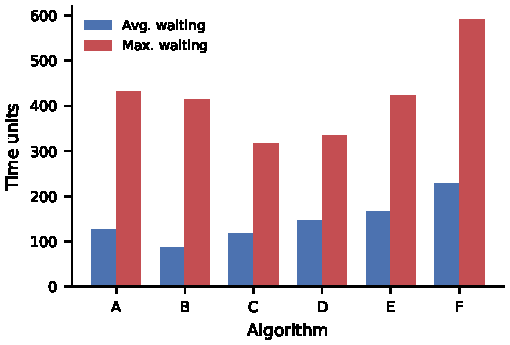
\includegraphics[width=0.95\linewidth]{fig_main_waiting.pdf}
\caption{Mean average and maximum waiting time by algorithm, across 65 paired test workloads.}
\label{fig:main}
\end{figure}

\subsection{Statistical Comparisons}
Table~\ref{tab:stats}: paired two-sided Wilcoxon signed-rank tests on per-workload average waiting time, Holm-corrected across the six-comparison family, with a percentile bootstrap (2{,}000 resamples) 95\% CI for the mean ratio.

\begin{table}[h]
\centering
\caption{Paired comparisons, average waiting time (Holm-corrected).}
\label{tab:stats}
\scriptsize
\setlength{\tabcolsep}{3.0pt}
\begin{tabular}{lrrrl}
\toprule
\textbf{Comparison} & \textbf{Ratio} & \textbf{95\% CI} & \textbf{$p_{\text{Holm}}$} & \textbf{Result} \\
\midrule
B vs.\ A & 0.68 & [0.62, 0.74] & $8.8\!\times\!10^{-10}$ & B faster \\
C vs.\ B & 1.35 & [1.21, 1.55] & $4.0\!\times\!10^{-7}$ & C slower \\
C vs.\ A & 0.92 & [0.86, 0.98] & $8.5\!\times\!10^{-5}$ & C faster \\
E vs.\ D & 1.13 & [1.06, 1.18] & $1.1\!\times\!10^{-3}$ & E slower \\
F vs.\ D & 1.55 & [1.46, 1.64] & $2.8\!\times\!10^{-11}$ & F slower \\
F vs.\ E & 1.37 & [1.32, 1.45] & $1.4\!\times\!10^{-11}$ & F slower \\
\bottomrule
\end{tabular}
\end{table}

Algorithm B reduced mean waiting time $32\%$ versus A, the strongest result here. C sits between A and B as designed: $35\%$ higher average waiting than B but $8\%$ lower than A, while cutting mean max-waiting from $431.7$ to $317.8$ ($-26\%$) versus A -- yet C's starvation-violation count ($12.2$) was \emph{not} lower than A's ($11.3$) or B's ($7.0$), consistent with the algorithm's own documented guarantee gap (\S IV-C): bounding the \emph{worst} wait is not the same as reducing the \emph{count} of threshold violations. Neither adaptive RR policy beat fixed-quantum RR: E was $13\%$ slower and F $55\%$ slower than D, both significant. We attribute this to the deliberately small pilot-scale search/training budgets (\S VII-F) rather than reading it as evidence that adaptive quantum selection is unhelpful in general, but we report it exactly as measured.

\subsection{CWABP vs.\ Exponential Averaging}
\begin{table}[h]
\centering
\caption{CWABP vs.\ exponential averaging (EA), mean over 10 seeds.}
\label{tab:cwabp}
\scriptsize
\setlength{\tabcolsep}{2.8pt}
\begin{tabular}{lrrrr}
\toprule
\textbf{Workload type} & \textbf{EA wait} & \textbf{CWABP wait} & \textbf{$\Delta$} & \textbf{RMSE EA$\to$CW} \\
\midrule
Stable & 59.0 & 58.2 & $-1.4\%$ & 4.35 $\to$ 4.38 \\
Feature, strong & 65.6 & 64.1 & $-2.3\%$ & 7.18 $\to$ \textbf{5.38} \\
Feature, moderate & 65.6 & 64.3 & $-2.0\%$ & 7.18 $\to$ 6.99 \\
Uncorrelated & 83.4 & 81.6 & $-2.1\%$ & 15.54 $\to$ 15.88 \\
Phase change & 171.1 & \textbf{161.3} & $\mathbf{-5.7\%}$ & 26.75 $\to$ 25.58 \\
Correlation break & 65.6 & 64.4 & $-1.8\%$ & 7.18 $\to$ 7.11 \\
Heavy-tailed & 31.2 & 30.8 & $-1.2\%$ & 12.09 $\to$ 12.16 \\
\bottomrule
\end{tabular}
\end{table}

\begin{figure}[h]
\centering
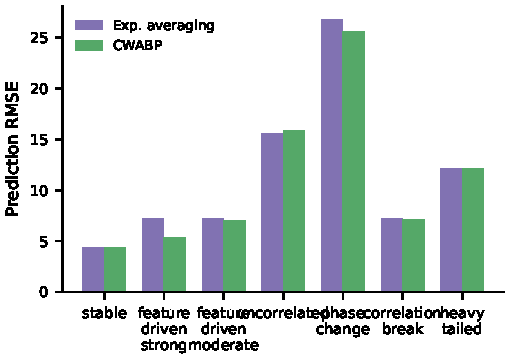
\includegraphics[width=0.95\linewidth]{fig_cwabp_rmse.pdf}
\caption{Burst-prediction RMSE, EA vs.\ CWABP, by workload type (mean of 10 seeds).}
\label{fig:cwabp}
\end{figure}

CWABP matched or modestly improved on EA in every tested condition, with the clearest wins on \emph{feature-driven, strong-correlation} (RMSE $-25\%$) and \emph{phase-change} ($-5.7\%$ waiting time) workloads, and small degradation ($<3\%$ RMSE) on the adversarial \emph{uncorrelated} and \emph{heavy-tailed} cases -- consistent with the trust-region clamp (Eq.~\ref{eq:clamp}) successfully preventing the spurious-correlation failure mode it was designed to guard against.


\section{Implementation and Reproducibility}

\subsection{Open-Source Simulator}
All six algorithms, five burst-prediction models, the Q-learning agent, and CWABP are implemented in \texttt{schedsim}, a Python package with no modification to any real kernel; the accompanying repository includes the exact code used to produce every table and figure above.

\subsection{Verification and Testing Suite}
Beyond empirical metrics, \texttt{schedsim} enforces structural invariants with two complementary layers. \textbf{42 unit/invariant tests} verify: $B(\alpha{=}1)\equiv A$ and $C$-with-safeguards-disabled $\equiv B$, both checked pid-for-pid across the dispatch event log, not merely metric-equal; $G{=}0\Rightarrow$ no priority inversion outside override events; structural absence of burst/priority/arrival leakage in feature matrices; Q-learning state indices bounded in $[0,144)$; a frozen policy is fully deterministic; and analytical bounds for turnaround ($T_i{=}W_i{+}b_i$), Jain's index ($\in[1/n,1]$), and starvation counts ($\in[0,n]$). \textbf{10 Hypothesis property-based suites} re-verify the same class of invariants, but over randomly generated and automatically shrunk inputs (process counts $2$--$40$, arbitrary seeds, all burst/arrival/priority modes, and arbitrary floating-point state inputs) rather than hand-picked cases, including a no-future-information property for CWABP that mutates a not-yet-observed burst's true length and asserts the prediction is unaffected.

\subsection{Continuous Training and Data Flywheel}
A separate CLI, \texttt{train.py}, lets the burst predictors and the Q-agent keep improving across repeated rounds rather than being refit once on a fixed batch. Each round: (i) an \textbf{append-only pool} (\texttt{schedsim/pool.py}) samples new workloads from seeds strictly disjoint from the evaluation splits and appends their processes to \texttt{training\_pool.csv}; (ii) \textbf{checkpointing} (\texttt{schedsim/checkpoint.py}) refits all five regression models on the accumulated pool, logs validation RMSE to a leaderboard CSV, and atomically promotes the best model to \texttt{predictor\_latest.pkl}; and (iii) the \textbf{Q-agent resumes} from a serialized Q-table (\texttt{qtable\_latest.npz}), continuing its $\varepsilon$-decay schedule from the cumulative episode count rather than restarting. On a 3-round smoke test (20 workloads/round, 200 episodes/round), validation RMSE improved monotonically ($22.27\to21.95\to21.79$) as the pool grew, and the Q-table's cumulative episode count correctly persisted across independent process invocations.

\subsection{Two Bugs This Project's Own Testing Caught}
Development surfaced two genuine correctness issues. First, an early CWABP multi-burst generator precomputed arrival times assuming no queueing contention; under real contention this let a process's \emph{own} next burst appear ready before its current one had finished simulating, inflating mean waiting time $\sim\!8\times$ before being fixed via online, completion-time-driven burst generation. Second, a small-window spurious correlation in CWABP could combine with an out-of-range feature value to overflow \texttt{math.exp}; an adversarial unit test caught this and it was fixed with the log-space trust-region clamp (Eq.~\ref{eq:clamp}). Both fixes are reflected in the numbers reported here, and the second is now additionally covered by a Hypothesis property test that searches the clamp's boundary directly.

\subsection{Threats to Validity}
\textbf{Internal.} Validation workloads are used twice (prediction and scheduler tuning), which can make validation estimates optimistic; the disjoint test split is never touched during either step. \textbf{External.} All workloads are synthetic with a known, designed feature-burst relationship; the main study assumes one burst per process with no I/O (CWABP relaxes this only for its own comparison). Absolute numbers should not be read as transferable to a real kernel -- only relative comparisons, and these remain preliminary at pilot scale. \textbf{Statistical.} Workloads within a category are similar by construction, so reported Wilcoxon tests describe this study's designed mixture, not external real-world traffic.

\subsection{Limitations and Future Work}
Results here are pilot-scale: smaller sample sizes, search/training budgets, and tuning grids than the full protocol, run via \texttt{-{}-full} or \texttt{-{}-deep} for a larger instance of the identical pipeline (\S VIII) with no change to the algorithms. Planned next steps: a full-scale run; validation against real process traces; a kernel-level prototype to measure real prediction overhead; deep Q-networks once the tabular baseline is well understood at scale; and multi-core scheduling, which this study does not address.

\section{Conclusion}
At pilot scale, ML-weighted priority scheduling (B) delivered a large, statistically robust reduction in mean waiting time, and its fairness-protected variant (C) delivered a smaller but positive reduction while substantially improving worst-case waiting -- though not, at this operating point, the count of starvation-threshold violations, a nuance the algorithm's own design does not rule out. Neither adaptive Round Robin variant beat the fixed-quantum baseline at this scale, reported without qualification. CWABP matched or modestly improved on exponential averaging across every tested condition, including adversarial ones, attributable to the trust-region safeguard added after the project's own tests surfaced a genuine failure mode. The continuous training flywheel demonstrates that both the predictor and the Q-agent can keep improving with more compute rather than being fixed at a single batch size.

\section*{Data and Code Availability}
The complete simulator, test suite, and scripts used to produce every result above are released under the MIT license. Structure: \texttt{schedsim/} (\texttt{workload.py}, \texttt{predictors.py}, \texttt{schedulers.py}, \texttt{qlearning.py}, \texttt{cwabp.py}, \texttt{pool.py}, \texttt{checkpoint.py}, \texttt{metrics.py}, \texttt{experiment.py}, \texttt{stats.py}); \texttt{tests/} (42 unit tests + \texttt{test\_properties.py}, 10 Hypothesis suites); \texttt{run\_experiment.py} (generates Tables~\ref{tab:main}--\ref{tab:cwabp}, Figs.~\ref{fig:main}--\ref{fig:cwabp}); \texttt{train.py} (continuous training flywheel); \texttt{paper/} (this \LaTeX{} source).

\begin{quote}\small\ttfamily
pip install -r requirements.txt\\
python run\_experiment.py --seed 0 \quad\# reproduce exactly\\
pytest tests/ -v \quad\# 52 tests\\
python train.py run --rounds 5 --workloads 50\\
python run\_experiment.py --deep \quad\# 20k+ Q-learning episodes
\end{quote}
No part of the pipeline requires network access, proprietary data, or a license beyond the open-source dependencies in \texttt{requirements.txt} (NumPy, SciPy, scikit-learn, pandas, Hypothesis).

\section*{Acknowledgment}
The authors thank Dr Sudhamani MJ for the plagiarism check on this manuscript, and for guiding and helping us throughout this work, as she is our professor and we are doing this under her supervision.

\balance
\begin{thebibliography}{9}
\footnotesize
\bibitem{silberschatz2013} A. Silberschatz, P. B. Galvin, and G. Gagne, \textit{Operating System Concepts}, 8th ed. Wiley, 2013.
\bibitem{dias2017} S. Dias et al., ``A machine learning approach for improving process scheduling: A survey,'' \textit{IJCTT}, vol. 43, no. 1, pp. 1--4, 2017.
\bibitem{negi2005} A. Negi and P. K. Kishore, ``Applying machine learning techniques to improve Linux process scheduling,'' in \textit{Proc. TENCON}, 2005.
\bibitem{helmy2015} T. Helmy, S. Al-Azani, and O. Bin-Obaidellah, ``A machine learning-based approach to estimate the CPU-burst time for processes in the computational grids,'' in \textit{Proc. AIMS}, 2015.
\bibitem{dash2016} A. R. Dash, S. K. Sahu, and S. K. Samantra, ``An optimized round robin CPU scheduling algorithm with dynamic time quantum,'' \textit{IJCSEIT}, vol. 5, no. 2, 2016.
\bibitem{tajwar2017} M. M. Tajwar et al., ``CPU scheduling with a round robin algorithm based on an effective time slice,'' \textit{J. Inf. Process. Syst.}, vol. 13, no. 4, pp. 941--950, 2017.
\bibitem{mostafa2020} S. M. Mostafa and H. Amano, ``Dynamic round robin CPU scheduling algorithm based on K-means clustering technique,'' \textit{Appl. Sci.}, vol. 10, no. 15, 2020.
\bibitem{khan2025} Z. I. Khan, M. Khan, and S. N. M. Shah, ``Agent-based adaptive dynamic round robin (AADRR) scheduling algorithm,'' \textit{IEEE Access}, vol. 13, pp. 18308--18324, 2025.
\bibitem{han2020} J. Han and S. Lee, ``Performance improvement of Linux CPU scheduler using policy gradient reinforcement learning for Android smartphones,'' \textit{IEEE Access}, vol. 8, 2020.
\bibitem{li2024} P. Li et al., ``Reinforcement learning for adaptive resource scheduling in complex system environments,'' arXiv:2411.05346, 2024.
\bibitem{watkins1992} C. J. C. H. Watkins and P. Dayan, ``Q-learning,'' \textit{Machine Learning}, vol. 8, no. 3--4, pp. 279--292, 1992.
\end{thebibliography}

\end{document}
